% !TEX root = /home/computer/ucsc/master-2/quarter-1/machine-learning/master.tex
\assignment{3}{Sun 07 Nov 2021 20:05}{Assignment 3}

\subsectionfont{\fontsize{10}{10}\selectfont}

\graphicspath{ {/home/computer/ucsc/master-2/quarter-1/machine-learning/assignment_03/figures/} }

\section{Problem 1}

Using the last $10\%$ of training data for testing, and then using $1\%, 2\%,
5\%, 10\%, 20\%, \text{ and}, 100\%$ of the remaining data to train, we plot
the accuracy as a function of the percentage used to train.

\begin{figure}[H]
  \centering
  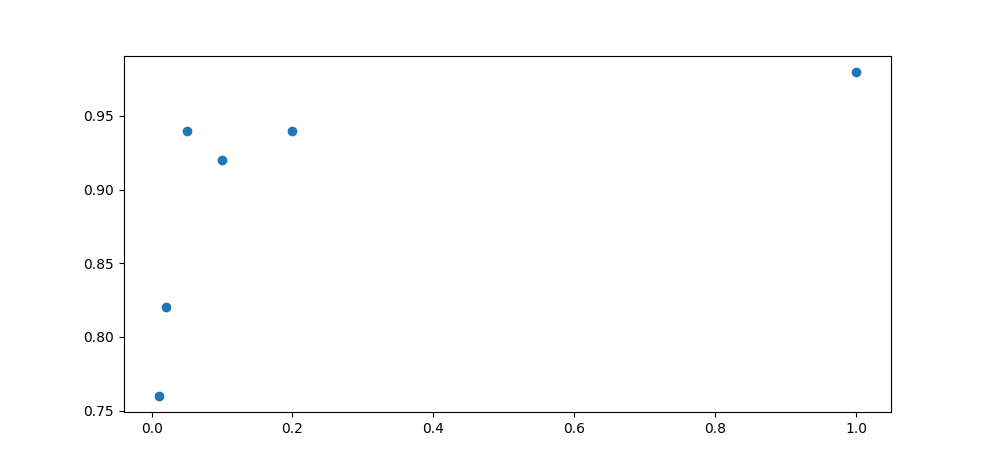
\includegraphics[width=0.8\linewidth]{Figure_1.png}
  \caption{Accuracy}%
  \label{fig:name}
\end{figure}

\section{Problem 2}
As the value of $k$ increases, the accuracy improves until we hit a plateau. So
we would want to pick the smallest k value that yields the greatest accuracy.
